\section{Methodology}
\label{sec:methodology}
The methodology for this thesis project stands on the development of a drone to use for the various tests and implementations, together with a controlled environment to test the drone in.
The development consists of hardware choices, software choices, and the constraints arising from these two, which dictate much of the design. 
\subsection{Design and Development}
\subsubsection{Flight Type}
A quadcopter design was a very clear choice as these are widely used and allow for very nimble and precise movement as opposed to fixed-wing designs which need to be in forward motion to generate upthrust for their flight. The Quadcopter design due to its symmetric nature make it very easy to predictably control it. 

On figure \autoref{fig:drone_movement} you can see standard quadcopter setup. If front motors ($m_1$, $m_2$) spin comparatively more the drone pitches up, if side propelers ( $m_1$, $m_4$) spin comparatively faster, then the drone rolls towards its left side, and thanks to the setup of alternating spin direction if propellers diagonally from each other fx $m_1$ and $m_3$ will spin faster, while $m_2$ and $m_4$ will spin slower the drone will turn on around in the direction of the propolers which are faster, in this case turn towards its left. This is given by Newton's first law as the inertia of propellers spinning faster will induce the rotation in the propellers' direction.
Opposingly, pitch and roll is achieved by spinning pairs of propellers on one side faster than on the other (left vs right, front vs back).
This makes the control of quadcopter somewhat simple as it can be summarized in a mathematical model.
\begin{figure}
    \centering
    \includegraphics[width=1\linewidth]{Figures/drone_movement_pareto.png}
    \caption{typical quadrocopter setup 'props-in', yaw $\psi$ (turning around), pitch $\theta$ (nose up or down) and roll $\phi$ (tilting to sides) From \cite{gomezParetoOptimalPID2020}}
    \label{fig:drone_movement}
\end{figure}
\subsubsection{Constraints and Design Objectives}
This work is a continuation of the Spinfly platform by A.~Lerche \cite{lercheSpinFlyUAVSystem}, which identified two primary limitations that directly shaped this project: \textbf{insufficient weight headroom}---the original platform struggled with takeoff when equipped with the protective cage, leaving no margin for component upgrades---and \textbf{insufficient battery capacity}, which created operational friction by limiting test throughput.

These problems are coupled: battery mass scales with capacity, yet a heavier battery forces higher motor output, accelerating discharge and potentially negating the added capacity. Solving both simultaneously required systematic trade-off analysis. Lerche also noted a lack of robust autonomous control and unreliable telemetry, which informed the autopilot selection.

From these constraints, three design targets were formulated:
\begin{enumerate}
    \item \textbf{Carry larger payloads} --- sufficient headroom for the cage and future instrumentation.
    \item \textbf{Achieve longer flight duration} --- extend mission time while maintaining efficient power draw.
    \item \textbf{Simplify autonomous control} --- adopt a proven, modular flight controller to reduce software complexity.
\end{enumerate}

\subsubsection{Platform Sizing: The 4-Inch Tradeoff}
\label{sec:sizing_tradeoff}

The drone's physical dimensions are governed by a narrow three-way tradeoff, illustrated in \autoref{fig:drone_sizing_tradeoff}:

\begin{figure}[htbp]
    \centering
    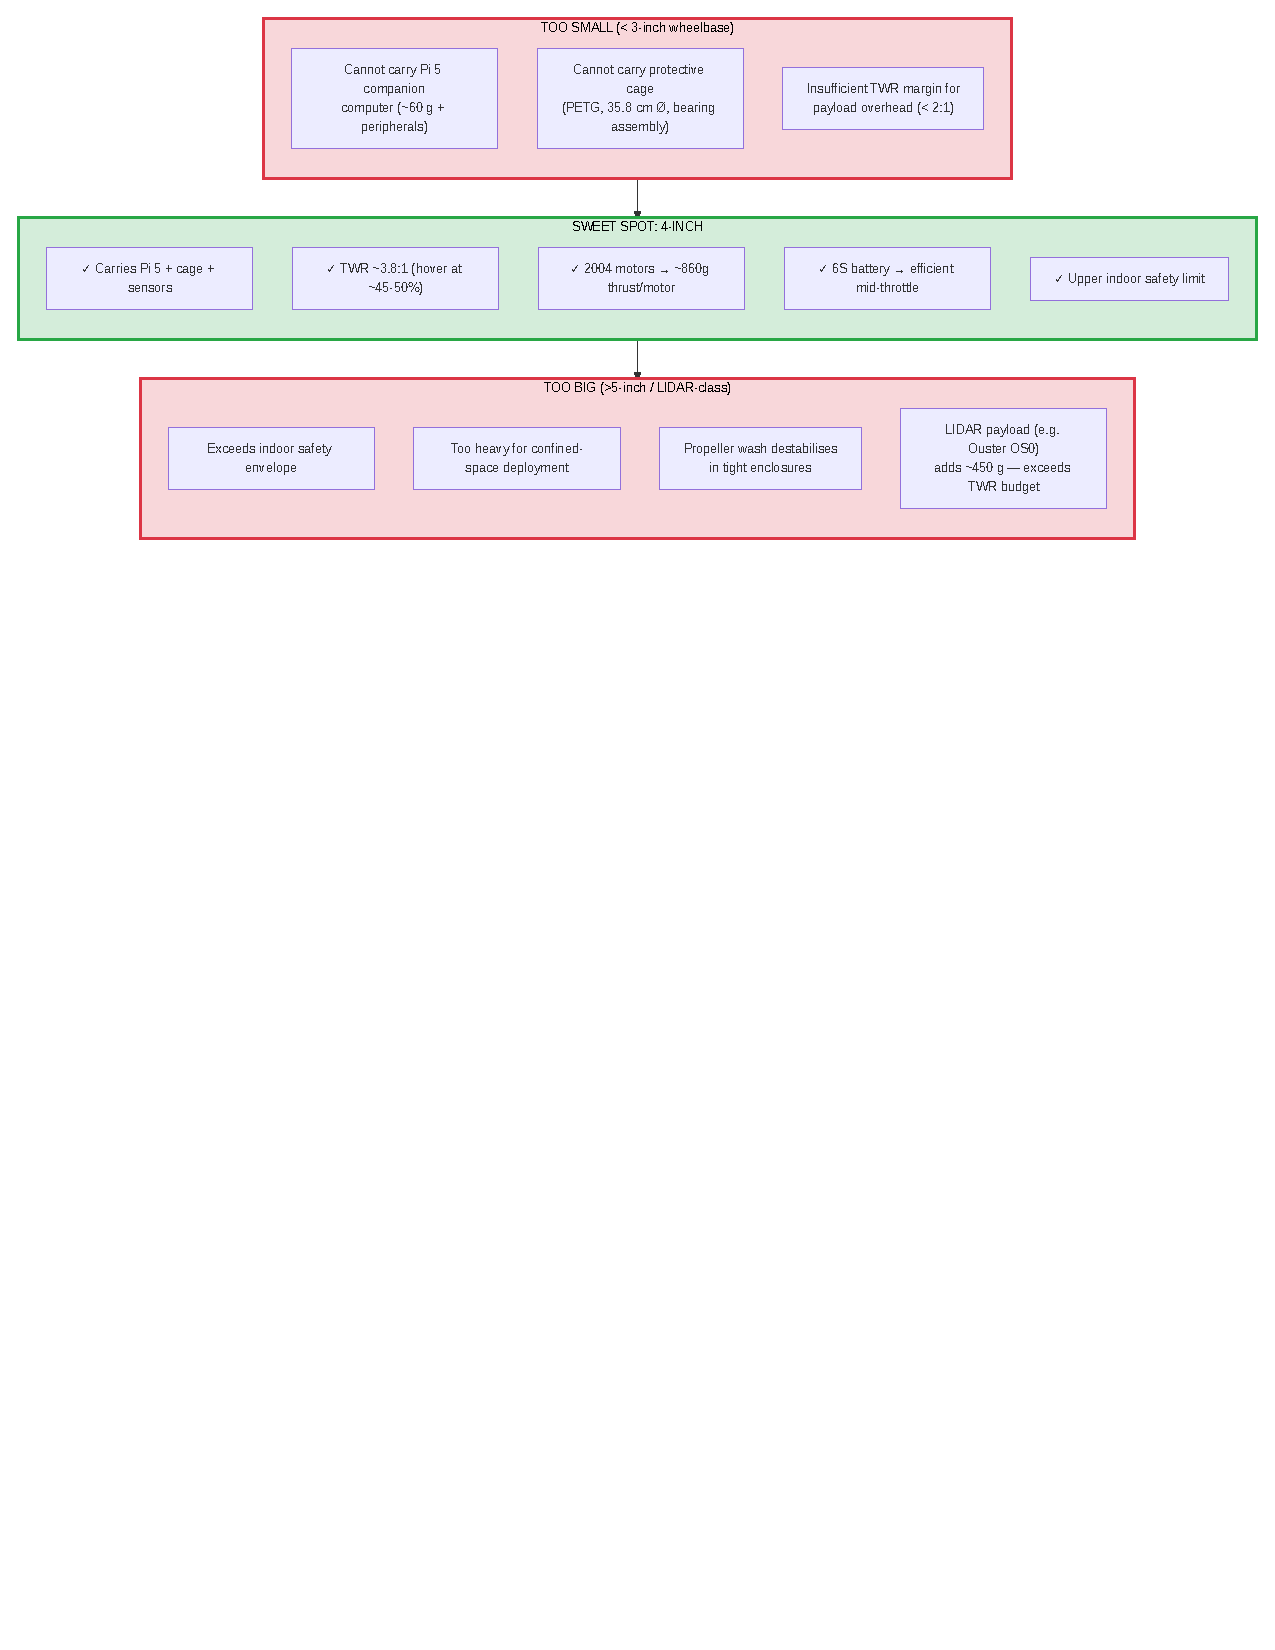
\includegraphics[width=0.95\textwidth]{Figures/drone_sizing_tradeoff.pdf}
    \caption{The three-way sizing constraint that defines the 4-inch platform: going smaller loses payload capacity; going larger violates indoor safety limits. The 4-inch wheelbase is the upper limit for confined indoor flight while providing sufficient thrust to carry the companion computer and protective cage.}
    \label{fig:drone_sizing_tradeoff}
\end{figure}

\textbf{Lower bound: payload minimum.} The Raspberry~Pi~5 companion computer ($\sim$60\,g plus peripherals) and the PETG (polyethylene terephthalate glycol, a 3D-printing filament) protective cage (35.8\,cm diameter, bearing assembly) together require a minimum thrust budget that class-3-inch and below platforms cannot provide. A typical 3-inch build lacks both the stator diameter and the propeller disc area to lift these components while maintaining a safe TWR (thrust-to-weight ratio) margin.

\textbf{Upper bound: indoor safety ceiling.} The 4-inch propeller class is the practical upper limit for indoor flight in confined spaces.\cite{FindYourPerfect} Larger platforms (5-inch and above) produce propeller wash that destabilises the vehicle in tight enclosures and increase the kinetic energy carried into any collision, raising the barrier to physical survivability. Platforms large enough to carry heavy sensors such as a full-size LIDAR (e.g., Ouster OS0 at $\sim$450\,g) exceed the thrust budget while also exceeding safe indoor operating dimensions.

\textbf{The 4-inch sweet spot.} At this scale, 2004-stator motors paired with 4-inch GF4023 propellers on a 6S battery produce sufficient lift for the companion computer and cage while hovering at 45--50\% throttle---near the efficiency peak. The resulting TWR of $\sim$3.8:1 places the drone in the responsive research-autonomy band, with enough thrust to arrest post-collision drift and recover to the commanded setpoint.

\paragraph{Platform Selection: PX4 and Pixhawk 6C}

To address these objectives holistically, PX4 was selected as the autonomous platform. Two platforms currently dominate the open-source UAV ecosystem: ArduPilot and PX4. PX4 was chosen over ArduPilot for its permissive BSD licensing (which allows proprietary extensions, whereas ArduPilot's GPLv3 requires contributed code to remain open), its modular publish-subscribe architecture (uORB), and its well-developed hardware standards under the Dronecode Foundation~\cite{meierPX4NodebasedMultithreaded2015}. PX4's open-source standard is built on modular architecture using \textbf{uORB (microObject Request Broker)}---a publish-subscribe middleware layer suited for plug-and-play development. These factors promised faster integration with the ROS~2 middleware layer and reduced hardware-software troubleshooting. This modularity enables rapid research iteration: novel autonomous behaviors can be implemented as independent modules without modifying the core flight stack.

The \textbf{Pixhawk 6C flight controller} was chosen as the hardware instantiation of the PX4 standard. Critically, Pixhawk is not a monolithic design but represents standardized connector specifications, sensor integration points, and reference schematics managed by the Dronecode Foundation~\cite{simpsonLatestPixhawkOpen2023}. This standardization means:

\begin{itemize}
    \item \textbf{Hardware swappability}: Sensors and peripheral electronics can be upgraded or replaced with components from different manufacturers (Holybro, ARK Electronics, CUAV) without redesigning integration.
    
    \item \textbf{Ecosystem maturity}: Over 1 million Pixhawk-based devices are deployed across commercial, research, and hobbyist applications.\cite{simpsonLatestPixhawkOpen2023}
    
    \item \textbf{Sensor integration}: The Pixhawk 6C includes integrated IMU and compass. Specifically, it features redundant inertial measurement units with onboard ICM-42688-P and BMI088 accelerometers/gyroscopes, plus an IST8310 magnetometer, with temperature-controlled operation via onboard heating resistors.\cite{TechnicalSpecificationHolybro2025, PX4Docs, Pixhawk6C6C} This eliminates the need for custom sensor fusion code---allowing focus on the research question rather than flight control tuning.
\end{itemize}

The 6C's form factor (84.8 \(\times\) 44 \(\times\) 12.4 mm) justifies the 4-inch drone design choice.\cite{TechnicalSpecificationHolybro2025} Four-inch platforms represent the upper practical limit for indoor flight while remaining large enough to carry meaningful payloads.

\paragraph{Thrust-to-Weight and Efficiency Rationale}

The design targets a \textbf{thrust-to-weight ratio (TWR) of approximately 3.8:1}, positioning the platform in the research/autonomous zone where hover occurs at roughly 45--50\% throttle. This mid-throttle hover is deliberate: motor efficiency peaks at 40--70\% throttle, and hovering at 50\% reserves substantial headroom for autonomous obstacle avoidance, gust rejection, and post-collision recovery. Hovering at or near 100\% throttle leaves zero control margin.\cite{oscarHowChooseFPV2024}

\paragraph{Motor and Battery Selection}

\textbf{EMAX ECOII 2004 1600KV} motors were selected. The 2004 stator (20\,mm diameter, 4\,mm height) provides high torque at mid-throttle while the low 1600\,KV rating (1600\,RPM per volt) is matched to a \textbf{6S LiPo battery} (22.2\,V nominal). On this voltage, the motors deliver approximately 860\,g static thrust each under 4-inch GF4023 propellers---a combined 3,440\,g.\cite{drone24hoursTMotorF20041700KV, oscarHowChooseFPV2024} The 6S voltage also places the practical RPM ($\sim$24,000--28,000 under load) within the 4-inch propeller's efficient range, avoiding excessive tip speeds.

\paragraph{Efficiency Advantage of 6S over 4S}

The choice of a 6-cell battery over a 4-cell alternative is driven by efficiency. At a given thrust level, higher voltage draws proportionally lower current, reducing resistive ($I^2R$) losses in the battery, ESCs, and motor windings. Empirically, 6S systems exhibit superior efficiency up to approximately 45\% throttle.\cite{recursionlabsRecursionLabs6s2021}

\textbf{Voltage sag}---the temporary voltage drop under high-current discharge, caused by battery internal resistance ($V_{\text{drop}} = I \times R_{\text{internal}}$)---is proportionally less severe at higher baseline voltages. Under an equivalent current spike, a 4S pack may sag by over 30\% of its nominal voltage, whereas an equivalent-quality 6S pack sees a smaller relative drop.\cite{oscarUsingLiPoBatteries2025} For autonomous flight, where the controller expects a predictable motor response, excessive sag introduces a latency between commanded and actual thrust that degrades control stability during rapid maneuvers. Higher baseline voltage provides a larger operating margin against this effect. The detailed derivation is given in the \hyperref[sec:annex_hardware]{Annex}.

\subsection{System Architecture}

The autonomous flight stack is organised into five layers, illustrated in \autoref{fig:architecture}: Hardware \& Firmware, Middleware, ROS~2 Environment, High-Level Control, and Data \& Analysis. Each layer was selected or developed to address the specific constraints of collision-resilient flight in signal-denied, confined spaces. An external Motion Capture subsystem and a standalone User Input node complete the architecture outside the layered stack.

\begin{landscape}
\begin{figure}[htbp]
    \centering
    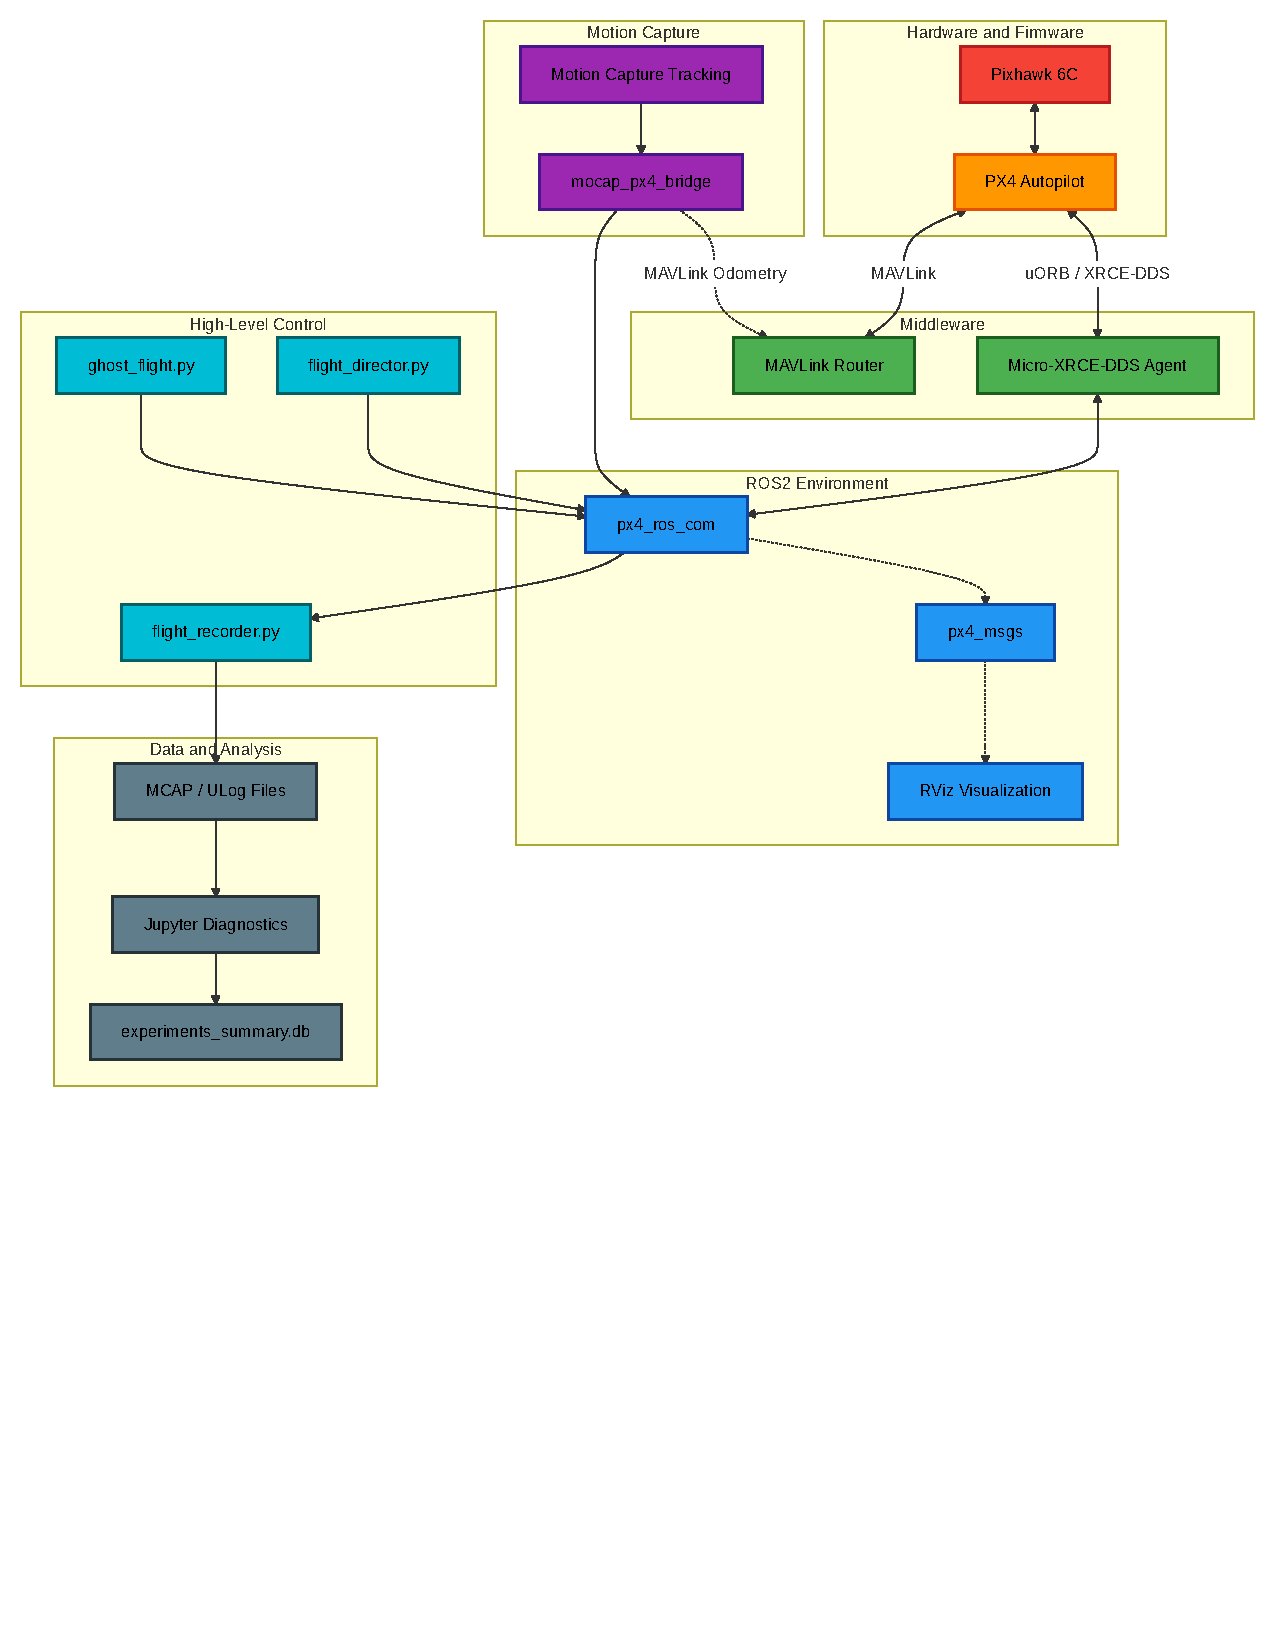
\includegraphics[width=1.45\textwidth]{Figures/architecture.pdf}
    \caption{Drone software stack architecture: PX4 flight controller (red), uXRCE-DDS middleware (green), ROS~2 environment (blue) with \texttt{px4\_msgs} flowing into \texttt{px4\_ros\_com}, high-level control nodes (teal) including the \texttt{flight\_director.py} state machine driven by Mission and User Input, and the data pipeline (grey) routing MCAP/ULog files through DB Pipeline to Experiment Summary and Jupyter Diagnostics. Motion capture (purple) enters via a Wi-Fi multicast link.}
    \label{fig:architecture}
\end{figure}
\end{landscape}

\subsubsection{Hardware Platform}

The companion computer is a \textbf{Raspberry Pi 5} running Ubuntu 24.04. It handles all high-level autonomy: waypoint navigation, MoCap data ingestion, offboard control logic, and telemetry logging. The Pi 5 communicates with the flight controller over UART (TELEM2) and mounts directly above it within the 4-inch frame envelope.

\subsubsection{Flight Controller}

The \textbf{Pixhawk 6C} runs PX4 Autopilot firmware (\texttt{v1.16.1rc}) and is responsible for low-level attitude control, motor mixing, and sensor fusion. Its dual IMU redundancy (ICM-42688-P and BMI088) and onboard IST8310 magnetometer are fused in the EKF2 estimator alongside external vision odometry from the MoCap system. The magnetometer is disabled for indoor operation to prevent interference with MoCap yaw data. The full parameter configuration is given in the repository \texttt{README.md}.

\subsubsection{Motion Capture Integration}

External state estimation is provided by an \textbf{OptiTrack Prime\textsuperscript{x}} 13-camera system streaming at 120\,Hz via NatNet. The \texttt{motion\_capture\_tracking} ROS 2 node receives the multicast stream, and the \texttt{mocap\_px4\_bridge} node transforms the poses from the MoCap ENU frame to PX4's NED/FRD convention, publishing them to \texttt{/fmu/in/vehicle\_visual\_odometry}. The EKF2 estimator fuses this external vision with the onboard 250\,Hz IMU data, bridging any MoCap tracking dropouts through inertial propagation.

\subsubsection{Communication Middleware}

The flight controller and companion computer communicate over a UART serial link (TELEM2, 921\,600 baud). During experimental flights, the link uses \textbf{uXRCE-DDS} exclusively: the PX4 uXRCE-DDS client publishes internal uORB topics (\texttt{vehicle\_odometry}, \texttt{vehicle\_status}, \texttt{actuator\_motors}) to the ROS 2 node graph via \texttt{MicroXRCEAgent} running on the Pi 5. A secondary \textbf{MAVLink} stream can be enabled on the same port for ground-station debugging (QGroundControl), but the two protocols are not used simultaneously during active data collection.

\subsubsection{Software Framework}

\paragraph{Source Submodules}

The ROS~2 workspace integrates several external repositories as Git submodules, providing the interface layer between the high-level autonomy code and the low-level PX4 flight stack:

\begin{lstlisting}[basicstyle=\ttfamily\footnotesize,numbers=none,caption={Source submodules under \texttt{src/} providing the ROS~2--PX4 interface layer.},label={lst:submodules}]
src/
  px4_msgs/                    # PX4 message definitions (uORB <-> ROS 2)
  px4_ros_com/                 # Frame transforms & utility libraries
  Micro-XRCE-DDS-Agent/        # uXRCE-DDS middleware bridge agent
  motion_capture_tracking/     # OptiTrack NatNet receiver node
  mocap_px4_bridge/            # ENU -> NED coordinate transformer
  PX4-Autopilot/               # PX4 firmware source (SITL builds only)
\end{lstlisting}

Three of these are critical for the MoCap-to-PX4 chain: \texttt{px4\_msgs} provides the interface message definitions (ROS~2 \texttt{.msg} files mirroring PX4 uORB topics), \texttt{px4\_ros\_com} handles frame transformations (ENU to NED/FRD), and \texttt{mocap\_px4\_bridge} publishes the transformed poses to \texttt{/fmu/in/vehicle\_visual\_odometry}.

\paragraph{The Flight Director}

The \texttt{flight\_director.py} node was developed directly from the PX4 ROS~Com offboard control examples, inheriting their structure for heartbeat publishing, offboard mode switching, and trajectory setpoint generation. It serves as the primary mission executor:

\begin{itemize}
    \item \textbf{State machine}: Implements the waypoint state machine shown in \autoref{fig:waypoint_state_machine}, transitioning through DISARMED $\to$ TAKEOFF (WP0) $\to$ WP\_stage (U-turn) $\to$ Exp.\ Start-point (WP1) $\to$ Exp.\ End-point (WP2) $\to$ Recovery (WP3) $\to$ (auto-loop to WP\_stage, or LANDING). Each state transition publishes a waypoint-identifier message that drives the event segmenter.
    \item \textbf{Offboard control}: Publishes \texttt{TrajectorySetpoint} messages to \texttt{/fmu/in/trajectory\_setpoint} with explicit velocity feedforward (\texttt{hb.velocity = True}). Subscribes to \texttt{/fmu/out/vehicle\_status} for telemetry feedback.
    \item \textbf{Safety enforcement}: Monitors the geofence boundary with the cage-radius offset (17.9\,cm) subtracted, and triggers an emergency landing on breach, MoCap loss, or spacebar kill-switch.
\end{itemize}

The complete experimental pipeline, from hardware through the ROS~2 node graph to telemetry storage, is illustrated in \autoref{fig:experiments_pipeline}.

\begin{figure}[htbp]
    \centering
    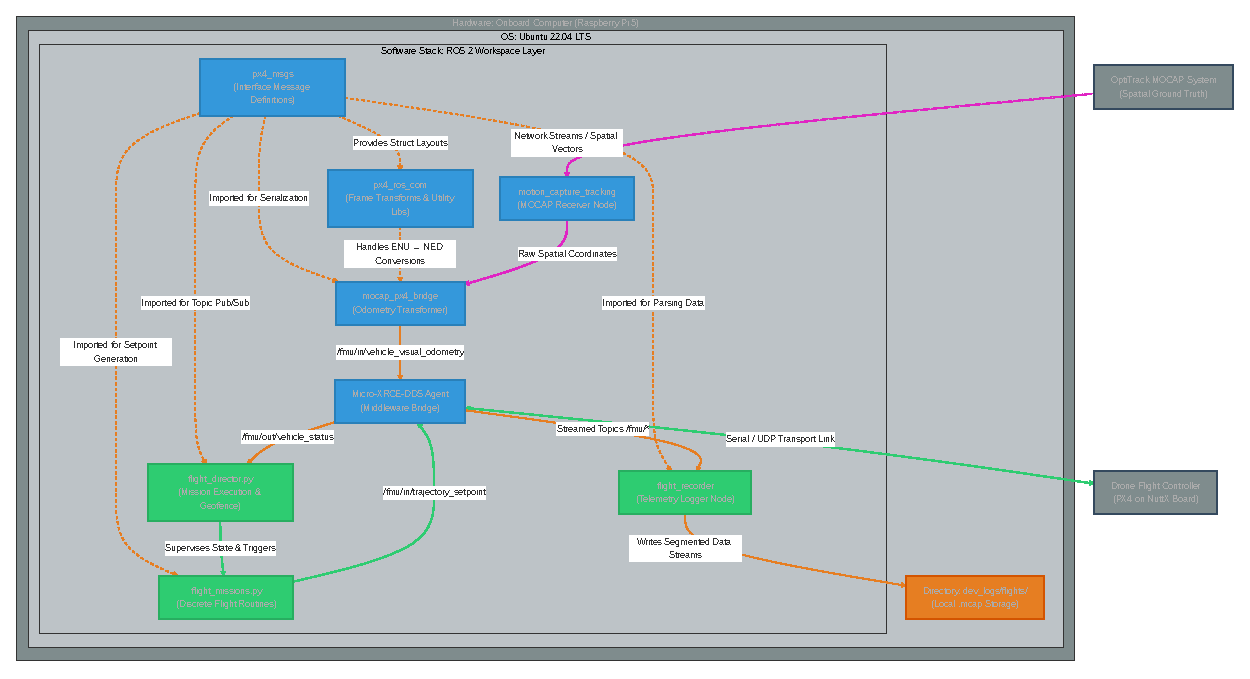
\includegraphics[width=\textwidth]{Figures/experiments_pipeline.pdf}
    \caption{Experiment pipeline showing hardware components, ROS~2 software stack, data flow from MOCAP through the agent to PX4, and telemetry logging to MCAP storage.}
    \label{fig:experiments_pipeline}
\end{figure}

The \texttt{flight\_missions.py} module provides discrete flight routines (column sweep, hover verification), while \texttt{flight\_recorder.py} logs synchronised topic data to segmented \texttt{.mcap} files, one per loop iteration.



\subsubsection{Frame and Cage Design}

The protective cage design draws on two established geometries from the collision-resilience literature. Mahmud et al.\cite{mahmudDevelopmentCollisionResilient2021} compared a freely rotating gimbal sphere against a G\"omb\"oc-shaped shell (a mono-monostatic body with a single stable equilibrium), concluding the turtle-like G\"omb\"oc form was superior for self-righting after impacts. The cage adopted for this work shares the rotating-shell principle: a PETG-printed spherical cage of 35.8\,cm diameter, mounted on a bearing assembly that allows the outer shell to spin freely upon contact with an obstacle. This mechanical decoupling converts linear collision momentum into rotational energy, shunting impact shock away from the central fuselage and flight controller.

The fixed-cage control configuration uses identical geometry but rigidly mounts the outer shell to the frame, eliminating the bearing's rotational degree of freedom. All other parameters (mass, diameter, material, propeller clearance) are held constant between the two configurations, isolating the effect of the bearing mechanism as the single experimental independent variable.

\